%==============================================
\section{Dimensioning a Tokamak}
%==============================================
From the previous equations mostly derived from a 0-dimensional approach (shaped profiles have not been considered so far), a suitable couple $(R, B)$ may be found for a given reactor project of prescribed $(P_{DT}, Q)$. By proceeding this way, some other characteristics of the plasma (namely the shape of the plasma, including elongation and aspect ratio, the average ion mass $\hat M$, the edge safety factor $q_a$ and the density $n_N$ normalised to the Greenwald density) are assumed to be prescribed by other considerations. Notice however that these other variables actually offer additional degrees of freedom to the exercise. The method is applied to the ITER case in section \ref{sec:ITER_spec}.

Should such a $(R, B)$ couple be found, additional important questions then arise before deciding whether it effectively constitutes a suitable tokamak. These includes, but are not limited to, the issues of superconducting magnets with their cryostat and neutron shielding, the issue of power exhaust and of the maximum affordable heat flux per square meter, the capacity to sustain a sufficiently long a plateau of plasma current...\\

%----------------------------------------------
\subsection{Recovering ITER specifications}
\label{sec:ITER_spec}

The objective here is to find a suitable couple of major radius and magnetic field $(R,B)$ which would allow one to reach the ITER targets in terms of fusion gain $Q=10$ and fusion power $\hat P_{DT}=410$ MW.
So as to get closer to the actual specifications of ITER, one should first refine the various constants introduced in section \ref{sec:governing_eqs}. One introduces the following refinements:
\begin{enumerate}
    \item $f_\alpha \doteq n_{He}/n_e$ the fraction of $\alpha$ particles
    \item $f_p \doteq \langle T^2 \rangle / \langle T \rangle^2$ the peaking factor of the temperature profile (a flat density profile is assumed). Here and hereafter in this section, the brackets $\langle ...\rangle$ refer to volume averaged quantities.
    \item $\theta_i \doteq T_i/T_e$ the ratio of ion to electron temperatures
\end{enumerate}
Several coefficients are modified by these additional variables:
\begin{eqnarray*}
    && C_{fus} \to C_{fus} \times (1-2f_\alpha)^2\theta_i^2 \times f_p \\
    && C_{loss} \to C_{loss} \times \frac{1+\theta_i - f_\alpha\theta_i}{2}  \\
    && C_\beta \to C_\beta \times \frac{1+\theta_i - f_\alpha\theta_i}{2}
\end{eqnarray*}
The corrections regarding $C_{fus}$ result from the fact that $P_{DT}$ scales like $\langle n_Dn_TT_i^2 \rangle$, with $n_D = n_T = 0.5\; (1-2f_\alpha)n_e$ so as to fulfill electro-neutrality ($n_D+n_T+2n_{He}=n_e$), and $\langle T_i^2 \rangle = f_p\; \langle T_i \rangle^2$ by definition. As expected, $\alpha$ particles are responsible for a dilution effect. The correction regarding $C_{loss}$ and $C_\beta$ is due to the fact that both the power loss and $\beta$ scale like the total pressure which reads: $\sum_s n_sT_s = n_eT_e (1+\theta_i- f_\alpha \theta_i)$ with the assumption that $T_\alpha=T_i$.
In addition, the effective mass $\hat M$ simply derives from $f_\alpha$\footnote{Indeed, one has: $(n_D+n_T+n_{He})\; \hat M \doteq n_D\hat M_D + n_T\hat M_T + n_{He}\hat M_{He} =
n_e\left\{ (\hat M_D + \hat M_T)(1-2f_\alpha)/2 + f_\alpha \hat M_\alpha \right\}$, with $\hat M_D=2$, $\hat M_T=3$ and $\hat M_\alpha=4$.}:
\begin{equation*}
    \hat M = \frac{5  - 2f_\alpha}{2(1-f_\alpha)}
\end{equation*}
Finally, geometrical effects modify the $C_I$ coefficient. When including the effect of triangularity $\delta$, the revised expression reads as follows (cf. eq.(17) in \cite{Johner2011}):
\begin{equation*}
    C_I \to C_I \times 
    \frac{(1.17-0.65\, \varepsilon)\; \left[ 1+\kappa^2(1+2\delta^2-1.2\delta^3) \right]} {2\;(1-\varepsilon^2)^2}
\end{equation*}

\begin{figure} 
	\begin{center}
		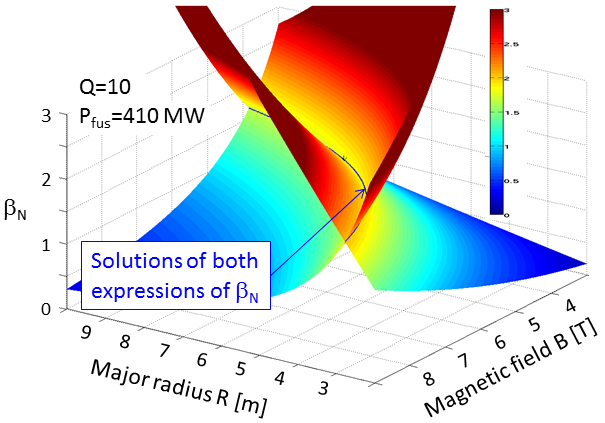
\includegraphics[width=0.8\textwidth]{figures/Fig_3D_betaN_R_B_ITER.png}
		\caption{Surfaces governed by eq.\ref{eq:DT_fusion_power_betaN} and eq.\ref{eq:nTtau_betaN} in the 
			3-dimensional $(\beta_N,R,B)$ space. Blue line: intersection of these 2 surfaces.}
		\label{fig:R_B_betaN_3D}
	\end{center}
\end{figure}

\begin{figure} 
	\begin{center}
		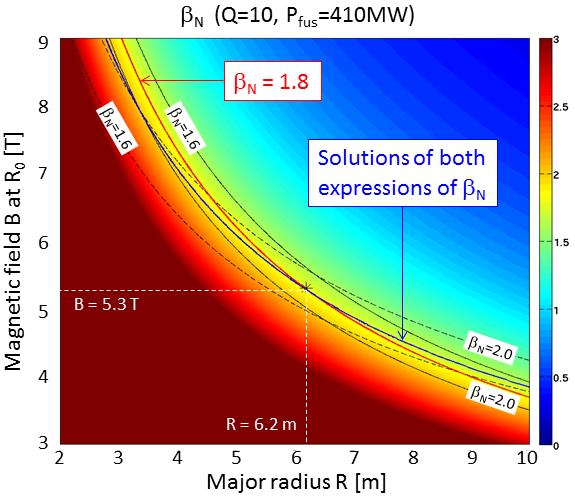
\includegraphics[width=0.7\textwidth]{figures/Fig_2D_betaN_R_B_ITER.png}%\hfill
		%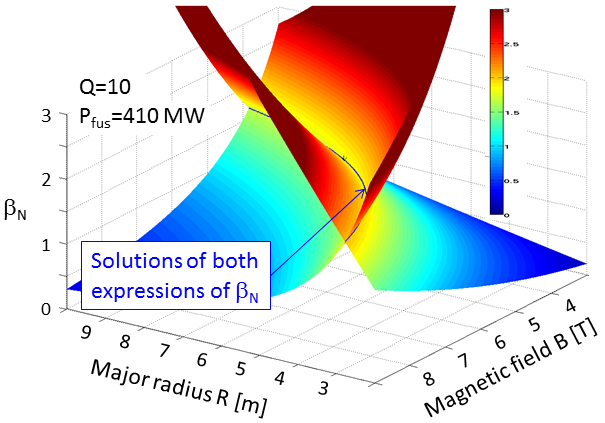
\includegraphics[width=0.5\textwidth]{figures/Fig_3D_betaN_R_B_ITER.png}
		\caption{Map of $\beta_N=f(R,B)$ given by eq.\ref{eq:DT_fusion_power_betaN} (color-scale and plain contour lines) and eq.\ref{eq:nTtau_betaN} (dashed contour lines). Blue line: intersection of these 2 surfaces. Red line: $\beta_N = 1.8$.}
		\label{fig:R_B_betaN_2D}
	\end{center}
\end{figure}

Hereafter, the following set of parameters has been considered, mostly taken from ref.\cite{Johner2011}\footnote{The chosen peaking factor would correspond, for instance, to the following temperature profile: $T = (T_0-T_a)*(1-\rho^2)^{1.41} + T_a$, with $\rho=r/a$, and $\hat T_a=0.1$ keV and  $\hat T_0=15$ keV the temperatures at the separatrix and on the magnetic axis, respectively.}:
\begin{center}
	\begin{tabular}{c|c|c|c|c|c|c|c}
		\hline
		$q_a$ & $\varepsilon^{-1}$ & $\kappa$ & $\delta$ & $n_N$ & $f_\alpha$ & $f_p$ & $\theta_i$ \\
		\hline
		$3$   & $3.1$ & $1.7$ & $0.33$ & $0.85$ & $0.1$ & $1.5$ & $1/1.25$ \\
		\hline	
	\end{tabular}
\end{center}
The approximate values of the various coefficients are then the following:
\begin{center}
	\begin{tabular}{c|c|c|c|c|c|c}
		\hline
		$C_{SL}$ & $C_n$ & $C_I$ & $C_\beta$ & $C_{loss}$ & $C_{fus}$ & $\hat M$ \\
		\hline
		$0.0562$ & $3.183$ & $13.144$ & $0.693$ & $0.082$ & $9.24\,10^{-4}$ & $2.67$ \\
		\hline	
	\end{tabular}
\end{center}
\bigskip

\begin{figure} 
	\begin{center}
		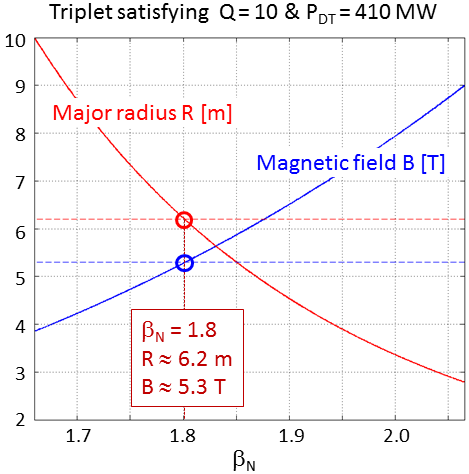
\includegraphics[width=0.5\textwidth]{figures/Fig_R_B_betaN_solutions.png}
		\caption{Values of $R$ and $B$ as a function of $\beta_N$ which fulfill both equations eq.\ref{eq:DT_fusion_power_betaN} and eq.\ref{eq:nTtau_betaN} (taken along the blue line of fig.\ref{fig:R_B_betaN_2D}). The solution at $\beta_N=1.8$ is close to the ITER specifications $R_{ITER}=6.2$m, $B_{ITER}=5.3$T.}
		\label{fig:solutions_betaN}
	\end{center}
\end{figure}

Two independent expressions of $\beta_N$ with respect to $R$ and $B$ are provided by equations eq.\ref{eq:DT_fusion_power_betaN} and eq.\ref{eq:nTtau_betaN}. The intersection of these 2 surfaces draws a line in the $(R,B,\beta_N)$ plane, as evident on Fig.\ref{fig:R_B_betaN_3D}. This line is plotted in blue on figures \ref{fig:R_B_betaN_3D} and \ref{fig:R_B_betaN_2D} (the latter figure being a projection of the former one). As expected, it does not follow an iso-$\beta_N$ contour (should it be the case, this would actually mean that the 2 equations are degenerate). Figure \ref{fig:R_B_betaN_2D} also shows the iso-contour lines $\beta_N \in \{1.6, 2\}$, which allow one to locate the ITER relevant region in the $(R,B)$ plane, i.e. those solutions exhibiting an acceptable $\beta_N$ value for ITER performing discharges. 
It readily appears from Fig.\ref{fig:R_B_betaN_3D} that $\beta_N$ given by eq.\ref{eq:DT_fusion_power_betaN} decreases with $(R,B)$, while eq.\ref{eq:nTtau_betaN} leads to the increase of $\beta_N$ with $(R,B)$, all other parameters being kept constant.
Noticeably, plain and dashed iso-contours look almost tangent to each other. This property implies that the set of couples $(R,B)$ which are solutions of the problem does not cover a broad range of $\beta_N$ values. This point is evident on fig.\ref{fig:solutions_betaN}, which displays the $(R,B)$ solutions as a function of $\beta_N$: for $\beta_N$ in the range $1.66 \leq \beta_N \leq 2.06$, the acceptable couples $(R,B)$ are in the range $2.78 \leq R_{[m]} \leq 10$ and $3.83 \leq B_{[T]} \leq 9$.

Interestingly, it turns out that the triplet $(R_{[m]},B_{[T]},\beta_N) = (6.2, 5.3, 1.8)$ is a possible solution of the problem\footnote{More precisely, the couple $(R_{[m]},B_{[T]}) = (6.21, 5.27)$ is solution at $\beta_N=1.8$.}. This set of parameters is consistent with ITER specifications.
